\documentclass[11pt, xcolor={dvipsnames}, hyperref={colorlinks, allcolors=Blue}]{beamer}


% Packages
\usepackage{graphicx}
\usepackage{caption, subcaption}
\usepackage{tikz}
\usepackage{amsmath, amsfonts, amssymb}
\usepackage{booktabs}
\usepackage{apacite}
\usepackage{multirow}
\usepackage{doi}
\usepackage{textpos}
\usepackage{lipsum}
\usepackage{amsfonts, amsmath}
\usepackage{wrapfig}
\usepackage{animate}
\usepackage{cleveref}


\renewcommand\doiprefix{}


\usepackage{tikz}
\usetikzlibrary{shapes, fit}





%%%%%%%%%%%%%%%%%%%%%%%%%%%%%%%%%%%%%%%%%%%%%%
% Custom commands
\newcommand\bc[1]{{\usebeamercolor[fg]{frametitle} {\textbf{#1}}}} % bold and color
\newcommand{\into}{\rightarrow}








%%%%%%%%%%%%%%%%%%%%%%%%%%%%%%%%%%%%%%%%%%%%%%
% Set CSIRO Theme
\usetheme{Boadilla}
\usecolortheme{rose}

%%%%%%%%%%%%%%%%%%%%%%%%%%%%%%%%%%%%%%%%%%%%%%
% Make citation font tiny
\renewcommand{\bibliographytypesize}{\tiny}

%%%%%%%%%%%%%%%%%%%%%%%%%%%%%%%%%%%%%%%%%%%%%%
% Fonts
\usefonttheme{serif} % Serif font
\setbeamertemplate{enumerate items}[default] % Don't use bullets in enumerate.

%%%%%%%%%%%%%%%%%%%%%%%%%%%%%%%%%%%%%%%%%%%%%%%
% Remove navigation bar
\setbeamertemplate{navigation symbols}{}
%%%%%%%%%%%%%%%%%%%%%%%%%%%%%%%%%%%%%%%%%%%%%%


% Frontmatter
\title[ECON 8000 -  Lecture 2]{Lecture 2: Real Analysis II}
\author[University of Queensland]{Robert Garrard}
\date[\today]{} 


%%%%%%%%%%%%%%%%%%%%%%%%%%%%%%%

% Common commands
\newcommand{\R}{\mathbb{R}}
\newcommand{\N}{\mathbb{N}}
\newcommand{\Z}{\mathbb{Z}}
\newcommand{\Q}{\mathbb{Q}}
\renewcommand{\P}{\mathbb{P}}
\newcommand{\E}{\mathbb{E}}

\renewcommand{\epsilon}{\varepsilon}

\renewcommand{\implies}{\Rightarrow}
\newcommand{\halmos}{\hfill$\blacksquare$}



\newcounter{Lecture}
\addtocounter{Lecture}{2}

\newcounter{exercise}
\newenvironment{exercise}[1][]{\refstepcounter{exercise}\par\medskip
   \noindent {\bc{Exercise}~\bc{\theLecture.\theexercise} #1}}{\medskip}
%%%%%%%%%%%%%%%%%%%%%%%%%%%%%%%%

% Tikz
\usetikzlibrary{arrows,shapes,trees, positioning}

%%%%%%%%%%%%%%%%%%%%%%%%%%%%%%


\begin{document}

\begin{frame}
\titlepage

\begin{picture}(0,0)
\put(35,-50){\hbox{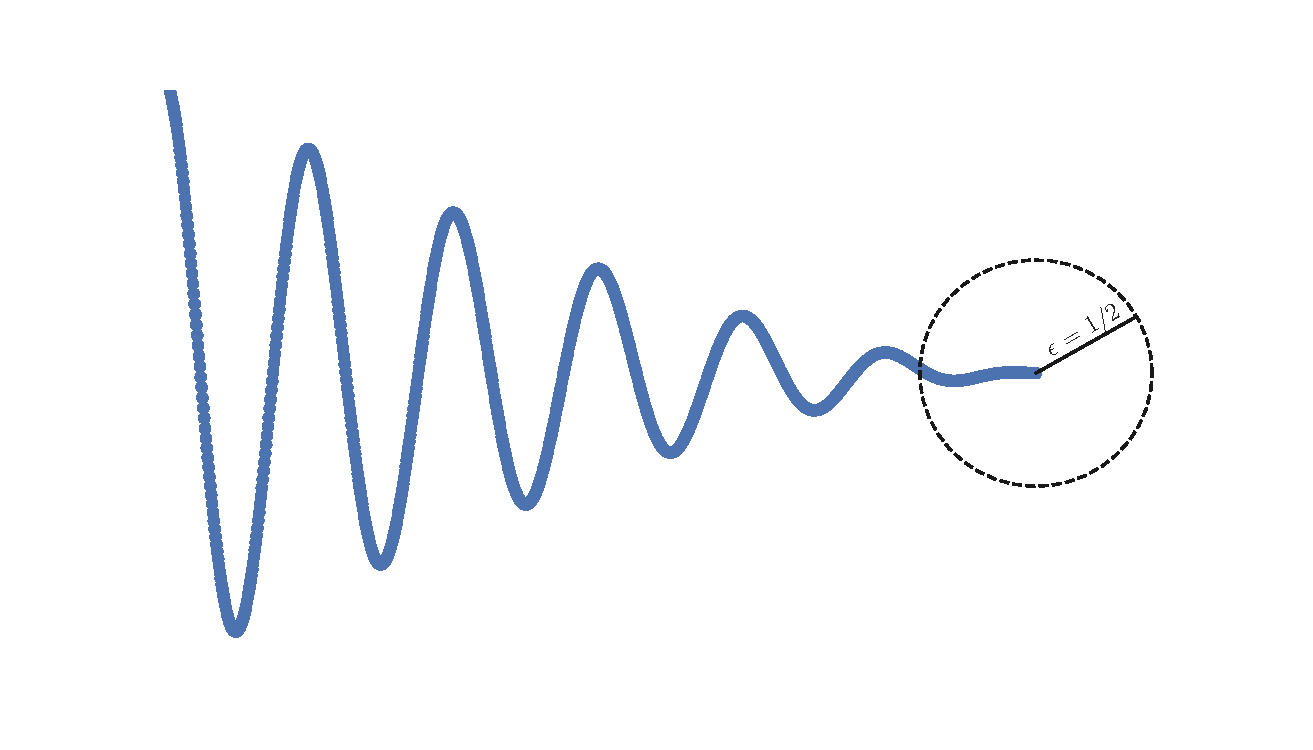
\includegraphics[width=0.8\textwidth, trim={0cm, 1cm, 0cm, 1cm}, clip]{convergence.pdf}}}
\end{picture}

%\centering
%	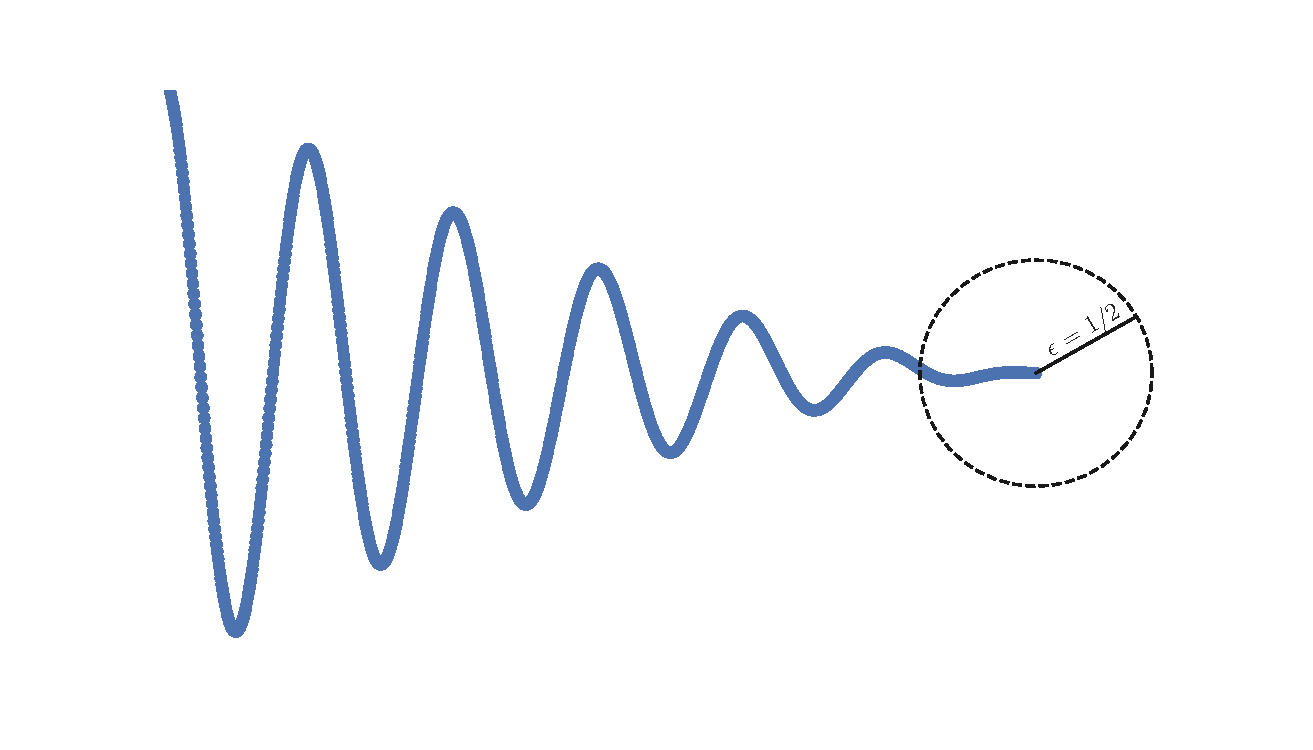
\includegraphics[width=0.8\textwidth]{convergence.pdf}

\end{frame}

%%%%%%%%%%%%%%%%%%%%%%%%%%%%%
\begin{frame}{Metric Spaces}

A \bc{space} is just a set endowed with some sort of structure.\\\bigskip

A \bc{metric space} is a set endowed with a notion of \bc{distance}.\\\bigskip

A metric space is a pair $(X,d)$ where $X$ is a set and\\ $d:X\times X \rightarrow \R$ is a function which satisfies the following conditions
\begin{enumerate}
\item $d(x,y) \geq 0 \ \  \forall x,y\in X \text{  and  } d(x,y) = 0 \Leftrightarrow x = y$

\item $d(x,y) = d(y,x) \ \ \forall x,y \in X$

\item $d(x,z) \leq d(x,y) + d(y,z) \quad \forall x,y,z \in X \ \ \text{(\emph{Triangle inequality})}$

\end{enumerate}


\end{frame}
%%%%%%%%%%%%%%%%%%%%%%%%%%%%%

\begin{frame}{Metric Spaces}

The metric we encounter most is the familiar \bc{Euclidean metric}, which is one way of defining distance between two points in $\mathbf{x}, \mathbf{y} \in \R^{n}$. Recall that the Euclidean metric is defined as

\[d(\mathbf{x}, \mathbf{y}) = \sqrt{(x_{1} - y_{1})^{2} + (x_{2} - y_{2})^{2} ... + (x_{n} - y_{n})^{2}}\]
\bigskip

\begin{exercise}
\begin{enumerate}
	\item Show that the Euclidean metric in $\R$, $d(x, y) = |x - y|$, is in fact a metric.

	\item Show that the \bc{discrete metric} is a metric.

\[d(x,y) = 
\begin{cases}
   0 & \text{if } x = y \\
   1  & \text{otherwise }
  \end{cases}
\]
\end{enumerate}
\end{exercise}
\end{frame}

%%%%%%%%%%%%%%%%%%%%%%%%%%%%%
%%%%%%%%%%%%%%%%%%%%%%%%%%%%%

\begin{frame}{Open and Closed Balls}

Equipped with a notion of distance, we can construct some useful objects in a metric space, $(X, d)$.\bigskip

An \bc{open ball} of radius $r > 0$ centered at $a$ is the set:

\[ B(a,r) = \{x \in X\ | \ d(x,a) < r\}\]

The \bc{closed ball} of radius $r>0$ centered at $a$ is the set

\[ \bar{B}(a,r) = \{x \in X\ | \ d(x,a) \leq r\}\]
\bigskip

\begin{exercise}
 What does an open/closed ball of unit radius, centered at the origin, look like in $\R^{2}$ under the:
\begin{enumerate}
	\item Euclidean metric?
	\item Discrete metric?

\end{enumerate}
\end{exercise}
\end{frame}


%%%%%%%%%%%%%%%%%%%%%%%%%%%%%

\begin{frame}{Sequences}

A \bc{sequence} is an ordered set of elements taken from some set, where the members of the sequence are indexed by the natural numbers.\bigskip

 Specific sequences are often written by enumerating the first few elements if there is an obvious pattern,  such as:

\begin{center}
`` the sequence $\{2,4,6,8,\dots\}$''
\end{center}

or by explicitly stating what the $n$th element of the sequence is, such as:

\begin{center}
 ``the sequence $\{x_{1}, x_{2}, x_{3},\dots\}$ where $x_{n} = 2n$''
\end{center}

An arbitrary sequence from some set $X$ is often written as $\{x_{n}\}_{n\in \N}$.

\end{frame}

%%%%%%%%%%%%%%%%%%%%%%%%%%%%%

\begin{frame}{Convergence of Sequences}

Consider the sequence $\{\frac{1}{1}, \frac{1}{2}, \frac{1}{3}, \frac{1}{4},\dots\}$. As $n$ becomes large, the elements in this sequence become very small. They get closer and closer to zero, although the sequence never actually attains this value at any time. We can use our metric to capture the notion of ``closeness'' to some limiting point of the sequence. \bigskip

A sequence, $\{x_{n}\}_{n \in \N}$, is said to \bc{converge} to a point $a$ if

\[\forall \epsilon > 0 \quad \exists N\in \N \ \ s.t \ \ \forall n > N \ \  d(x_{n}, a) < \epsilon\]


We often write this proposition as $\lim_{n\to\infty} x_{n} = a$ or $x_{n} \to a$.\bigskip

An sequence which does not converge to any point is said to \bc{diverge}.

\end{frame}

%%%%%%%%%%%%%%%%%%%%%%%%%%%%%
\begin{frame}{Convergence of Sequences}

If that definition is tricky to parse, let's try to English it up a little:\bigskip

For a sequence to converge to some point, $x_{n} \to a$, it must be that if I place a ball at $a$ of \emph{any} radius, then \emph{all but finitely many} elements of $x_{n}$ must be inside that ball.

\end{frame}


%%%%%%%%%%%%%%%%%%%%%%%%%%%%


\begin{frame}{Convergence of Sequences}

\begin{block}{Example}
Show that the sequence $x_{n} = \frac{1}{n}$ for $n\in\N$ converges to 0 in the metric space $(\R, d)$, where $d$ is the Euclidean metric.\bigskip

Strategy: 
\begin{enumerate}
\item Pick an arbitrary $\epsilon > 0$.
\item Make a good choice for $N$ (as a function of $\epsilon$). 
\item Show that $n>N \implies |x_{n} - 0| < \epsilon$. \quad (eqv. $n>N \implies x_{n} \in B(0, \epsilon)$
\end{enumerate}
\bigskip

Pick some $\epsilon > 0$. Choose N to be any integer such that $N > \frac{1}{\epsilon}$. Consider some $n\in \N$. We have:\\

$n > N \implies n > \frac{1}{\epsilon} \implies \frac{1}{n} < \epsilon \implies x_{n} < \epsilon \implies |x_{n} - 0| < \epsilon$ (by non-negativity of $x_{n}$).\\

$\therefore x_{n} \to 0$\\
\hfill\halmos
\end{block}
\end{frame}


%%%%%%%%%%%%%%%%%%%%%%%%%%%%%
\begin{frame}{Convergence of Sequences}

\begin{exercise}
\begin{enumerate}
	\item Show that the sequence $\{1, 1, 1, 1, \dots \}$ converges to 1 under the discrete metric.
	\item Show that the sequence $\{0,1,0,1,0,1, \dots\}$ does not converge under the Euclidean metric.
\end{enumerate}
\end{exercise}
\end{frame}

%%%%%%%%%%%%%%%%%%%%%%%%%%%%%

\begin{frame}{Monotone Sequences}
A sequence $\{x_{n}\}$ in $\R$ is \bc{bounded} if
\[ \exists M\in R \ \  s.t \ \ |x_{n}| \leq M \ \forall n \in \N\] 

\begin{block}{Monotonicity}
A sequence $\{x_{n}\}$ in $\R$ is called
\begin{itemize}
\item[] \bc{Monotone Increasing} if $x_{n+1} \geq x_{n} \ \ \forall n\in \N$
\item[] \bc{Monotone Strictly Increasing} if $x_{n+1} > x_{n} \ \ \forall n$
\item[] \bc{Monotone Decreasing} if $x_{n+1} \leq x_{n} \ \ \forall n$
\item[] \bc{Monotone Strictly Decreasing} if $x_{n+1} < x_{n} \ \ \forall n$
\end{itemize}
\end{block}
\end{frame}

%%%%%%%%%%%%%%%%%%%%%%%%%%%%%

\begin{frame}{Monotone Sequences}

\begin{theorem}[Monotone Convergence Theorem]
A monotone sequence of real numbers converges iff it is bounded.\\

Further, if it is increasing (resp. decreasing), it converges to its supremum (infimum).
\end{theorem}

\textit{Proof.}\\


(Bounded $\implies$ converges, increasing case)\smallskip


Let $\{a_{n}\}$ be an increasing bounded sequence of real numbers. By the LUB property, $c = \sup \{a_{n}\}$ exists. \medskip

$\forall \epsilon > 0$ $\exists N$ sufficiently large that $a_{N} > c - \epsilon$, otherwise $c - \epsilon$ would be a smaller lower bound.\medskip

Since $a_{n}$ is increasing and $c$ is an upper bound: $\forall n \geq N$ $|a_{n} - c| \leq |a_{N} - c| < \epsilon$.\medskip

$\therefore$ $a_{n} \to c $.

\halmos

\vfill
\end{frame}


%%%%%%%%%%%%%%%%%%%%%%%%%%%%%

\begin{frame}{Cauchy Sequences}

A sequence $\{x_{n}\}$ is called a \bc{Cauchy sequence} if:

\[ \forall \epsilon > 0 \ \exists N\in \N \text{ s.t. } \forall m,n > N \ d(x_{m}, x_{n}) < \epsilon\]
\smallskip
In English: terms of the sequence must get \emph{closer together} as the sequence progresses and \emph{stay} close.

\begin{block}{Example}
Show that $x_n = \frac{1}{n}$ is Cauchy.\bigskip

For any $\epsilon$, we need to find an $N\in\N$ such that $|\frac{1}{m} - \frac{1}{n}| < \epsilon$ when $m,n > N$. Note that $\frac{1}{m} < \frac{1}{N}$, and similarly for $n$. \medskip

$|\frac{1}{m} - \frac{1}{n}| \leq |\frac{1}{m}| + |\frac{1}{n}| < \frac{1}{N} + \frac{1}{N} = \frac{2}{N} < \epsilon$
\medskip

Setting $N > \frac{2}{\epsilon}$ achieves the inequality.
\end{block}

\vfill\vspace{\fill}
\end{frame}

%%%%%%%%%%%%%%%%%%%%%%%%%%%%%

\begin{frame}{Cauchy Sequences}

\begin{theorem}[Cauchy Convergence Criterion]
A sequence of real numbers is convergent iff it is Cauchy
\end{theorem}
\bigskip

In general, convergent $\implies$ Cauchy. (Tutorial exercise)\bigskip

But in general Cauchy need not imply convergent.\bigskip

Usually we won't be trying to prove that a specific sequence converges to a specific value. Instead we'll be considering some sequence with a particular property, and be interested in whether it converges and, if so, what the properties of its limit point are.\bigskip

So we need some generic conditions under which convergence is guaranteed.

\vfill\vspace{\fill}
\end{frame}



%%%%%%%%%%%%%%%%%%%%%%%%%%%%%

\begin{frame}{Open and Closed Sets}


A set $X$ is \bc{open} if

\[\forall x \in X \quad \exists \epsilon > 0 \ \ s.t \ \ B(x,\epsilon) \subseteq X\]

That is, for any point in the set, there is some open ball centered at that point whose radius is sufficiently small for the ball to be entirely contained within the set.\bigskip

A set $X$ is \bc{closed} if its complement is open.\bigskip

Sets are not like doors! A set can be both open and closed.

\end{frame}

%%%%%%%%%%%%%%%%%%%%%%%%%%%%%

\begin{frame}{Open and Closed Sets}

\begin{block}{Some useful properties:}
\begin{itemize}
	\item The union of any collection of open sets is open.
	\item The intersection of any collection of closed sets is closed.
\smallskip
	\item The intersection of a finite collection of open sets is open.
	\item The union of a finite collection of closed sets is closed.
\end{itemize}
\end{block}

\end{frame}
%%%%%%%%%%%%%%%%%%%%%%%%%%%%%


%%%%%%%%%%%%%%%%%%%%%%%%%%%%%
\begin{frame}{Open and Closed Sets}

\begin{exercise}
\begin{enumerate}
	\item For a metric space $(X, d)$, show that the whole space $X$ is both open and closed.
	\item Show that a single point, $\{x\}$, is a closed set.
	\item Show that an open ball is an open set.
\end{enumerate}
\end{exercise}
\end{frame}

%%%%%%%%%%%%%%%%%%%%%%%%%%%%%
\begin{frame}{Open and Closed Sets}

\begin{block}{Proposition: Closed sets contain their limit points}
Let $(X, d)$ be a metric space. If $A\subseteq X$ is a closed subset and $a_{n}\in A$ is a sequence, then
$$a_{n} \rightarrow a \implies a \in A$$
\end{block}

Proof (tutorial exercise)
\end{frame}
%%%%%%%%%%%%%%%%%%%%%%%%%%%%%
\begin{frame}{Completeness}

\begin{exercise}

Let $(\Q, d)$ be a metric space over the rationals where $d$ is the Euclidean metric, $d(x, y) = |x - y|$. Let $A\subseteq \Q$, $A = \Q \cap [0, 2]$.
\begin{enumerate}
	\item Show that $A$ is closed.
	\item Does the sequence $x_{1} = 1$, $x_{n+1} = \frac{x_{n}}{2} + \frac{1}{x_n}$ converge?
\end{enumerate}
\end{exercise}

\end{frame}
%%%%%%%%%%%%%%%%%%%%%%%%%%%%%
\begin{frame}{Completeness}

A metric space, $(X, d)$, is \bc{complete} if \emph{every} Cauchy sequence converges.\bigskip

Every Euclidean space with the Euclidean metric, $(\R^{n}, d)$, is complete.\bigskip

\begin{block}{Proposition: Closedness preserves completeness}
If $(X, d)$ is a complete metric space and $A\subseteq X$ is a closed subset, then every Cauchy sequence in $A$ converges in $A$.
\end{block}

\end{frame}
%%%%%%%%%%%%%%%%%%%%%%%%%%%%%
\begin{frame}{Compactness}
An \bc{open cover} for a set $X$ is a (possibly infinite) collection of open sets, $\{A_{i}\}$, whose union contains $X$: $\bigcup_{i} A_{i} \subseteq X$.\bigskip

A set is called \bc{compact} if \emph{every} open cover has a finite sub-cover. \bigskip

\begin{theorem}[Heine-Borel]
A subset of $\R^{n}$ is compact iff it is closed and bounded.
\end{theorem}

\begin{exercise}

Which of the following subsets of $R$ are compact?
\begin{itemize}
	\item $(-\infty, 0]$
	\item $(0, 1)$
	\item $[0, \pi] \cap [0, e]$
\end{itemize}
\end{exercise}
\end{frame}
%%%%%%%%%%%%%%%%%%%%%%%%%%%%%
\begin{frame}{Compactness}
\begin{block}{Some properties of compactness}
	\begin{itemize}
		\item A compact metric space is complete.
		\item A closed subset of a compact set is compact.
		\item A compact subset of $R$ has a maximum and minimum value.
	\end{itemize}
\end{block}
\vfill\vfill
\end{frame}

%%%%%%%%%%%%%%%%%%%%%%%%%%%%%




\begin{frame}{Continuity}
A function, $f:X\into Y$, is \bc{continuous} at a point $c\in X$ if\bigskip

\bc{$\epsilon - \delta$ Continuity} \\
$\forall \epsilon > 0 \ \ \exists \delta > 0 \ \ s.t \ \ d(x,c)<\delta \implies d\left(f(x), f(c)\right) < \epsilon$
\bigskip

\bc{Sequential Continuity}\\
$\forall \{x_{n}\} \quad x_{n} \into c \implies f\left(x_{n}\right) \into f(c)$
\bigskip

\bc{Topological continuity}\\
$\text{Every open image, } V \text{, has an open preimage } f^{-1}(V)$
\bigskip

These definitions (and many others) are equivalent in a metric space. \bigskip

A function is called continuous if it is continuous at every point  in its domain.

\end{frame}
%%%%%%%%%%%%%%%%%%%%%%%%%%%%%
%%%%%%%%%%%%%%%%%%%%%%%%
\begin{frame}{Continuity}

\begin{block}{Some Properties}
\begin{itemize}
	\item Function composition preserves continuity.
	\item Continuous functions preserve compactness.
\end{itemize}
\end{block}

\begin{theorem}[Weirstrass Extreme Value Theorem]
Let $f:X\to Y$ be a continuous function and $X$ be a compact set. $f$ attains a maximum and a minimum.
\end{theorem}

\begin{theorem}[Intermediate Value Theorem]
Let $I = [a, b]$ be a closed interval and $f:I\to \R$ a continuous function. \\

If there is a $u$ such that $\min\{f(a), f(b)\} < u < \max\{f(a), f(b)\}$ then there exists a $c\in (a, b)$ st $f(c) = u$.
\end{theorem}
\end{frame}


%%%%%%%%%%%%%%%%%%%%%%%%%%%%%
\begin{frame}{Economic Application: Utility Representation}
Let $(X, \succsim)$ be a weak preference relation. Define this relation to be $\bc{continuous}$ if the following sets are closed:

\begin{align*}
&\{y \in X \ | \ y \succsim x\} \ \text{(upper contour set)}\\
&\{y \in X \ | \ x \succsim y\}\ \text{(lower contour set)}
\end{align*}


\begin{theorem}[MWG 3.C.1]
Suppose that the rational preference relation $\succsim$ on $X$ is continuous. Then there is a continuous utility function $U(x)$ that represents $\succsim$.
\end{theorem}


\end{frame}

\begin{frame}{Economic Application: Utility Maximization}

Let $\mathcal{B}(\mathbf{p}, w) = \{\mathbf{x} \in \R^{n}_{+} \ | \ \mathbf{x}\cdot \mathbf{p} \leq w\}$ be an agent's budget set, and let $U:\R^{n}\to\R$ be a continuous utility function.\bigskip

Show that the utility maximization problem
\begin{align*}
&\underset{\mathbf{x}}{\max} \ U(\mathbf{x}) \\
& \text{s.t. } \mathbf{x} \in \mathcal{B}
\end{align*}

has a solution. \bigskip

\textit{Proof}:\\
$\mathcal{B}$ is a closed and bounded subset of $\R^{n}$, therefore it is compact. The image of $\mathcal{B}$, $U(\mathcal{B})$ is also compact, since continuity preserves compactness. Compact subset's of $\R$ contain a maximum and minimum, so a solution exists.

\end{frame}

%%%%%%%%%%%%%%%%%%%%%%%%%%%%%
\begin{frame}{Contraction Mappings}

Let $(X, d)$ be a metric space. A function $f:X\to X$ is called a \bc{contraction mapping} if there exists an $ \  0\leq M < 1$ s.t. $\forall x, y \in X$, 

$$d\left( f(x), f(y) \right) \leq M d(x,y)$$

$M$ is called the \bc{modulus} of contraction.\bigskip

\begin{block}{Example}
Show that $f:\R\to \R$, $f(x) = \frac{1}{2}x$ is a contraction mapping.\\

$|\frac{1}{2}x - \frac{1}{2}y| = |\frac{1}{2}(x-y)| = \frac{1}{2}|x - y| \leq \frac{1}{2}|x - y|$\\

$\therefore f \text{ is a contraction mapping with } M=\frac{1}{2}$.
\halmos
\end{block}
\end{frame}

%%%%%%%%%%%%%%%%%%%%%%%%%%%%%
\begin{frame}{Contraction Mappings}

A function $f:X\to X$ has a \bc{fixed-point} if $\exists x\in X$ s.t. $f(x) = x$.\bigskip

\begin{theorem}[Banach Fixed-point Theorem]
Let $(X, d)$ be a non-empty complete metric space with a contraction mapping $f:X\to X$. Then $f$ admits a unique fixed-point $x^{*}$, $f(x^{*})=x^{*}$.\medskip

Furthermore, $x^{*}$ can be found by iterating $f$ on an arbitrary initial value. 
\end{theorem}
\bigskip

\begin{exercise}

What's the unique fixed-point of $f:\R \to \R$, $f(x) = \frac{1}{2} x$?

\end{exercise}
\end{frame}

%%%%%%%%%%%%%%%%%%%%%%%%%%%%%
\begin{frame}{Learning Outcomes}

\bc{You should be able to}:

\begin{itemize}
	\item Use properties of metric spaces, and open/closed balls in proofs.
	\item Determine whether a sequence is convergent, divergent, and prove that a sequence converges to a given point.
	\item Apply the monotone convergence theorem and Cauchy convergence criterion.
	\item Prove that a set is open, closed, both, or neither.
	\item Define a complete metric space.
	\item Use the Heine-Borel theorem to identify compact sets.
	\item Apply the Weirstrass and contraction mapping theorems.
\end{itemize}

\bc{You need not be able to}:
\begin{itemize}
	\item Prove that a particular function is continuous.
	\item Prove that a particular function is a contraction mapping.
\end{itemize}

\end{frame}

%%%%%%%%%%%%%%%%%%%%%%%%%%%%%



\end{document}















%%%%%%%%%%%%%%%%%%%%%%
\end{document}